%\documentclass{article}

%\usepackage{tikz}
%\usepackage[utf8]{inputenc}
%\usepackage[ngerman]{babel}
%\usepackage{color}
%\usepackage[a4paper,lmargin={2cm},rmargin={2cm},
%tmargin={2.5cm},bmargin = {2.5cm}]{geometry}
%\usepackage{amssymb}
%\usepackage{amsmath}
%\usepackage{graphicx}
%\usepackage{multicol}
%\usepackage{amsthm}

%\newtheorem*{defi*}{Definition}
%\newtheorem*{defi2*}{Definition}

%\begin{document}
%\begin{multicols*}{2}
\subsection{Norm und Skalarprodukt}
\author{Vivien Thi, Max Braun, Luca Bohn}
\begin{Def}
$||v||$ ist eine Norm im Vektorraum $V$ falls
\begin{enumerate}
\item 
\begin{enumerate}
\item $||v|| \geq 0$ für alle $v \in V$
\item $||v|| = 0$ nur für $v = 0$
\end{enumerate}
\item $||u+v|| \leq ||u|| + ||v||$ für alle $v \in V$
\item $|| \lambda v|| = |\lambda| ||v||$ für alle $\lambda \in \mathbb{R}$ und $v \in V$
\end{enumerate}
\end{Def}
Eine Norm kann nie negativ sein, ist die Norm 0 bedeuted das, dass der Vektor der Nullvektor ist. Wenn man zwei Vektoren
addiert, ist die Norm des resultierenden Vektors genau die Summe der Normen der beiden Ausgangsvektoren. Außerdem ist die
Norm eines Vektors, der mit einem reelen Faktor multipliziert wurde gleich dem Produkt aus der Norm des Vektors und dem 
Betrag des Faktors.

\begin{Def}
$f:V\times V \rightarrow\mathbb{R}$ ist ein Skalarprodukt wenn\\
\begin{enumerate}
\item $\left\langle  \alpha u + \beta v, w\right\rangle = \alpha \left\langle  u,w\right\rangle + \beta \left\langle  v,w\right\rangle $ (Bilinearität)
\item $\left\langle  u,v\right\rangle = \left\langle  v,u\right\rangle $ für alle $u,v \in V$
\item $\left\langle  v,v\right\rangle \geq 0$ mit $\left\langle  v,v\right\rangle = 0$ nur für $v = 0$\\
\end{enumerate}
\end{Def}
 

Üblicherweise wird das Skalarprodukt mit der folgenden Formel berechnet.

\begin{equation*}
\left\langle u,v\right\rangle  = u_1 v_1 + \dots + u_n v_n
\end{equation*}

An der ausgeschriebenen Form lässt sich überprüfen, ob es sich per Definition dabei wirklich um ein Skalarprodukt handelt. In der ausgeschriebenen Form wird aus $\left\langle \alpha u + \beta v, w\right\rangle $ dabei $(\alpha u_1 + \beta v_1) w_1 + \dots + (\alpha u_n + \beta v_n) w_n$. Durch Ausmultiplizieren der Produkte erhalten wir die Form $\alpha u_1 w_1 + \beta v_1 w_1 + \dots + \alpha u_n w_n +\beta v_n w_v$. Wenn wir daraus nach zwei Summen sortieren und die Summanden mit $\alpha$ von denen mit $\beta$ trennen können, wir die beiden Faktoren ausklammern und gelangen zu der aus der Definition geforderten Form $\alpha \left\langle u,w\right\rangle  + \beta \left\langle v,w\right\rangle $.\\
Die zweite Bedingung können wir mit dem Kommutativgesetz beweisen, wenn wir dieses auf die ausgeschriebene Form anwenden.
Für die dritte Bedingung ergibt sich $v_1 v_1 + \dots + v_n v_n = v_1^2 + \dots + v_n^2$. Da durch das Quadrieren keiner der Summanden kleiner als 0 werden kann und auch nur für $v_i = 0$ genau 0 werden kann, ist auch diese Bedingung erfüllt.\\


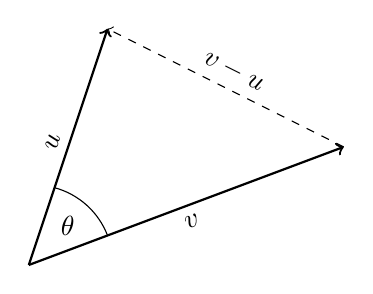
\begin{tikzpicture}
\coordinate (A) at (0,0);
\coordinate (B) at (4,1.5);
\coordinate (C) at (1,3);
\draw[thick, ->] (A) -- (B) node[pos=0.5,sloped,below]{$v$};
\draw[thick, ->] (A) -- (C) node[pos=0.5,sloped, above]{$u$};
\draw[dashed, ->] (B) -- (C) node[pos=0.5,sloped, above]{$v-u$};
\draw (1,0.375) arc (21:75:1);
\node[] at (45:0.7) {$\theta$};
\end{tikzpicture}

Da grundsätzlich $\left\langle v,v\right\rangle  = ||v||^2$ gilt, kann über die Abbildung auch die Aussage getroffen werden, dass $||v-u||^2 = \left\langlev-u,v-u\right\rangle $. Mit der Bilinearität des Skalarproduktes und der eben getroffenen Aussage können wir die Gleichung zu 
\begin{equation*}
||v-u||^2 = ||v||^2 - 2\left\langle v,u\right\rangle  + ||u||^2 
\end{equation*}
umformen.
Zusätzlich folgt aus dem Kosinussatz, dass $||v-u||^2 = ||u||^2 + ||v||^2 - 2 ||u|| ||v|| \cos\theta$. Setzt man beide Terme gleich, gelangt man über einige wenige Umformungen zu der Form $\left\langle u,v\right\rangle  = ||u|| ||v|| \cos\theta$, was ebenfalls eine Möglichkeit ist, das Skalarprodukt darzustellen.\\
Aus dieser Gleichung ergibt sich direkt die Cauchy-Schwarz Ungleichung. Da der Betrag des Kosinus sich nur zwischen 0 und 1 bewegt, gilt $\left\langleu,v\right\rangle  \leq ||u|| ||v||$.\\
Eine häufig genutzte Norm ist die Euklidische Norm, welche mit $||v||_2 = \sqrt{v_1^2 + \dots + v_n^2}$ definiert ist. Mit den zuvor getroffenen Aussagen können wir beweisen, dass es sich bei der Euklidischen Norm wirklich um eine Norm handelt.\\
Die erste und die dritte Bedingung aus der Definition für eine Norm zeigen sich aus der ausgeschriebenen Form der Euklidischen Norm. Da alle Komponenten dabei quadriert werden und die Wurzel gezogen wird muss die erste Bedingung stimmen. Ein Faktor $\lambda$, der ebenfalls quadriert in der Wurzel steht kann aus der Summe ausgeklammert werden und als Faktor vor die Wurzel gelangen. Der Betrag ergibt sich dabei daraus, dass $\lambda$ nach dem Vorgang nur positiv sein kann, auch wenn es zuvor negativ war.\\
Um zu beweisen, dass $||u+v|| \leq ||u|| + ||v||$ formen wir diese Ungleichung zu der bekannten Cauchy-Schwarz Ungleichung um. Hierzu quadrieren wir zunächst beide Seiten, ersetzen die quadrierten Normen durch Skalarprodukte und erhalten 
\begin{equation*}
|\left\langle u+v,u+v\right\rangle | \leq \left\langle u,u\right\rangle  + 2 ||u|| ||v|| + \left\langle v,v\right\rangle 
\end{equation*}
Die linke Seite der Ungleichung kann aufgrund der Bilinearität als $|\left\langle u,u\right\rangle | + 2 |\left\langle u,v\right\rangle | + |\left\langle v,v\right\rangle |$ geschrieben werden. Dadurch können wir auf beiden Seiten $|\left\langleu,u\right\rangle |$ und $|\left\langle v,v\right\rangle |$ subtrahieren und kommen so auf $||u+v|| \leq ||u|| + ||v||$, womit bewiesen ist, dass die Euklidische Norm eine Norm ist.

%\end{multicols*}
%\end{document}